%%%%%%%%%%%%%%%%%%%%%%%%%%%%%%%%%%%%%%%%%
% Friggeri Resume/CV
% XeLaTeX Template
% Version 1.0 (5/5/13)
%
% This template has been downloaded from:
% http://www.LaTeXTemplates.com
%
% Original author:
% Adrien Friggeri (adrien@friggeri.net)
% https://github.com/afriggeri/CV
%
% License:
% CC BY-NC-SA 3.0 (http://creativecommons.org/licenses/by-nc-sa/3.0/)
%
% Important notes:
% This template needs to be compiled with XeLaTeX and the bibliography, if used,
% needs to be compiled with biber rather than bibtex.
%
%%%%%%%%%%%%%%%%%%%%%%%%%%%%%%%%%%%%%%%%%
\documentclass[]{friggeri-cv} % Add 'print' as an option into the square bracket to remove colors from this template for printing

\usepackage{multicol}
\usepackage{lipsum}
\usepackage{graphicx}
\DeclareGraphicsExtensions{.pdf,.png,.jpg}


\begin{document}

\header{Jordi}{ Coscolla}{Full Stack Lead Developer} % Your name and current job title/field

%----------------------------------------------------------------------------------------
%	SIDEBAR SECTION
%----------------------------------------------------------------------------------------

\begin{aside} % In the aside, each new line forces a line break
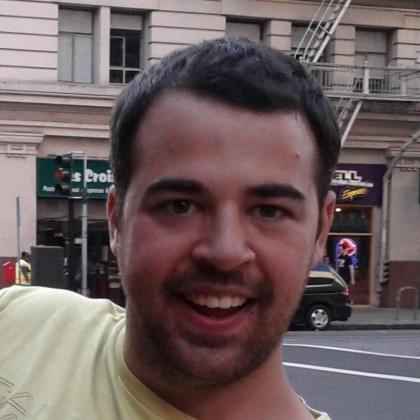
\includegraphics[width=3.6cm]{photo}
\section{Contact}
Capitan Arenas 64, 6-2
Barcelona, 08034 
Spain
~
+34 654 44 88 59
~
\section{Github/ Blog/ Mail}
\href{mailto:kozko2001@gmail.com}{kozko2001@gmail.com}
\href{http://github.com/kozko2001}{github.com/kozko2001}
\href{http://www.coscolla.net}{http://coscolla.net}
\href{http://stackoverflow.com/users/1021445/jordi-coscolla}{stackoverflow profile}
\section{Languages}
English, Spanish, Catalan
\section{Programming}
{\color{red} $\varheartsuit$} Scala, Kotlin, Python, Swift, Machine Learning,
React, TypeScript
\end{aside}

%----------------------------------------------------------------------------------------
%	EDUCATION SECTION
%----------------------------------------------------------------------------------------


\section{Experience}
\begin{entrylist}
%------------------------------------------------
\entry
{2017-2020}
{ThoughtWorks - Tech Lead}
{}
{
  ThoughtWorks is a consultancy firm with strong believe in iterative practices
  and tech excelence, working on different projects were I learn and grow.
\\

  Worked in multiple projects, from creating forms for ingesting new listings
  for market places, to implementing a wallet (ReactNative) for a research project focus
  on distributed ledgers for private data, and also building hardware pipelines
  for a media centers of cars.
\\

  Most of the challenges during this period were around using best practices on
  a variaty of projects, building high performing teams in challenging
  situations and being always in contact with remote part of the team.
}
\\
\entry
{2011--2017}
{UserZoom - Mobile leader}
{}
{
  Lead of the Mobile team at Userzoom, we had two main products that were
  developed in bot platforms (iOS and Android).

\vspace{\parsep}
\begin{itemize}
\item \emph{True Intent library}: A library to obtain feedback from the user
  after some particular flow of the app, capturing all kind of events including
  recording the screen.

\vspace{\parsep}
\item \emph{Task Based Mobile}: An app that was designed to make remote UX
  research of mobile web pages, simulating a browser clients were able to tests
  new prototypes, getting latter all the data (like clickstreams, different
  flows and screen recording).
\vspace{\parsep}
\end{itemize}
\vspace{\parsep}
Some of the clients were: \emph{Google, Paypal, Amazon etc...}\\
\vspace{\parsep}Technologies: \textbf{Objective-C, Android, Kotlin, Git, React}
} 
\\
%------------------------------------------------
\entry
{2010-2011}
{Force Manager - Mobile developer}
{}
{
ForceManager is a product oriented company that is developing apps to help to
manage the sales force allowing to have catalogs on phone/tablets or check which
customers have meet. I was responsable for the android app and also for part of the .NET backend.
\\\vspace{\parsep}Technologies: \textbf{Android, git, .NET}
}
\\
\entry
{2009-2010}
{CRIC (Centre de Recerca de Catalunya - Computer vision}
{}
{
As part of SignSpeack team, an European research project, aiming to translate
sign language video to natural language.
\\\vspace{\parsep}Technologies: \textbf{Python, openCV, C++}
}
\\
%------------------------------------------------
\entry
{2005-2009}
{Mapgenia}
{}
{
Help mining data to build dashboards for big pharmaceutical companies like MSD, Bristol
\\\vspace{\parsep}Technologies: \textbf{.Net, SQL Server, MS Reporting Services}
}
%------------------------------------------------
\end{entrylist}

%----------------------------------------------------------------------------------------
%	AWARDS SECTION
%----------------------------------------------------------------------------------------

\section{Education}

\begin{entrylist}
%------------------------------------------------
\entry
{2004--2009}
{University {\normalfont Computer Science}}
{FIB (Facultat d'Informàtica de Barcelona}
{Degree project: Commercials detection system for television. The user was
  notified when the TV shows resumes.


  Technologies: \textbf{.Net, SQL Server, MS Reporting Services}
}
%------------------------------------------------
%% \entry
%% {2002--2003}
%% {Bachelor {\normalfont speciality in Technology}}
%% {IES - Joan Fuster}
%% {}
%------------------------------------------------
\end{entrylist}

%----------------------------------------------------------------------------------------
%	WORK EXPERIENCE SECTION
%----------------------------------------------------------------------------------------

\section{Aptitudes}

%\begin{entrylist}
%------------------------------------------------

%Comion&\parbox[t]{11.8cm}{ \textbf{"HHH"}\hfill{"HOLA"}} \\
\begin{tabular}{p{3cm}p{10.8cm}}
\textbf{Communication} & mastery of the language to develop my ideas and express both to the technical team and to the final customer.
\vspace{\parsep}
\\
\textbf{Fast learning} & Deep knowledge of much of the new technologies and also
ease for learning.
\vspace{\parsep}
\\
\textbf{New challenges} & My behavior is based on mark me new goals to better and advance professionally.
\vspace{\parsep}
\\
\textbf{Team work} & Always beeing a peaceful person and empathy with everybody,
always try to bring the best of each other.
\vspace{\parsep}
\\
\end{tabular}


%\entry
%{Communication}{}{}
%{}
%\entry
%{Fast learning}{}{}
%\entry
%{New challanges}{}{}
%{}
%%------------------------------------------------
%\end{entrylist}

%----------------------------------------------------------------------------------------
%	COMMUNICATION SKILLS SECTION
%----------------------------------------------------------------------------------------

%\section{Technical Skills}
%
%\begin{multicols}{2}
%HOLA ?
%\vfill
%\columnbreak
%hola...
%\end{multicols}
%\begin{entrylist}
%%------------------------------------------------
%\entry
%{2011}
%{Oral Presentation}
%{California Business Conference}
%{Presented the research I conducted for my Masters of Commerce degree.}
%%------------------------------------------------
%\entry
%{2010}
%{Poster}
%{Annual Business Conference, Oregon}
%{As part of the course work for BUS320, I created a poster analyzing several local businesses and presented this at a conference.}
%%------------------------------------------------
%\end{entrylist}

%----------------------------------------------------------------------------------------
%	INTERESTS SECTION
%----------------------------------------------------------------------------------------

\section{Interests}


\begin{tabular}{p{3cm}p{10.8cm}}
\textbf{Professional} & <3 all tech stacks, Machine Learning, TDD, Python, Agile methodologies, emacs, git
\vspace{\parsep}
\\
\textbf{Personal} & Cooking, reading, running, beers
\vspace{\parsep}
\\
\end{tabular}

%----------------------------------------------------------------------------------------
%	PUBLICATIONS SECTION
%----------------------------------------------------------------------------------------


\end{document}
